\documentclass{article}

\usepackage{listings}
\usepackage{color,courier}
\usepackage[utf8]{inputenc}
\usepackage{graphicx}
\usepackage[top=20mm,bottom=20mm,left=45mm,right=30mm]{geometry}
\usepackage{courier}

\begin{document}

\lstset{
   language=C,
   title=\lstname,
   basicstyle=\ttfamily\normalsize\bfseries,%
   %
   showstringspaces=false,
   breaklines=true,
   numbers=left,
   numberstyle=\tiny\color[rgb]{0.7,0.7,0.7},
   numbersep=5pt,%
   %
   keywordstyle=\color[rgb]{0,0,0.5},
   backgroundcolor=\color[rgb]{1,1,1},
   commentstyle=\color[rgb]{0.9,0.045,0.033},
   stringstyle=\color[rgb]{1,0.1,0.1},
   literate={á}{{\'a}}{1}
            {é}{{\'e}}{1}
            {í}{{\'i}}{1}
            {ó}{{\'o}}{1}
            {ú}{{\'u}}{1}
            {ñ}{{\~n}}{1}
            {$}{{\$}}{1}
}

{\Large\bfseries
\hspace*{45mm}
Tareas
\newline
\newline
\newline
Díaz Urbina Eduardo
\newline
\newline
Boleta: 2012630487
\newline
\newline
Grupo: 1CV13
\newline
\newline
\newline
}
{\center\Large\bfseries
\hspace*{45mm}
Tarea (búsqueda)
\newline
\newline
}
a) Escribir un programa que realice una búsqueda
secuencial en una lista lineal vinculada en la
que se puedan ingresar y eliminar datos. Debe incluir
las mejoras de mover al frente y transposición, si un
elemento se ha buscado más de tres veces, se aplica
mover al frente, de lo contrario se aplica transposición.
\lstinputlisting{Busqueda/TareaA.c}
Capturas de Pantalla de Busqueda/TareaA.c
\newline
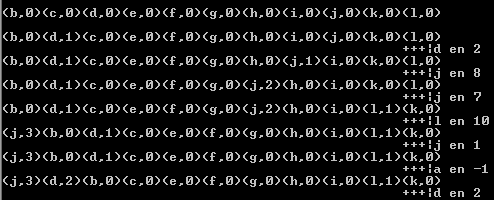
\includegraphics{Busqueda/img/TareaA_1.png}

\newpage
b) Hacer un programa para encontrar un elemento dentro
de un arreglo usando búsqueda binaria, cada elemento del
arreglo contiene la siguiente información: nombre, apellido
paterno, apellido materno, boleta y promedio; la búsqueda se
puede hacer tomando como llave cualquiera de estos elementos.
\lstinputlisting{Busqueda/TareaB.c}
Capturas de Pantalla de Busqueda/TareaB.c
\newline
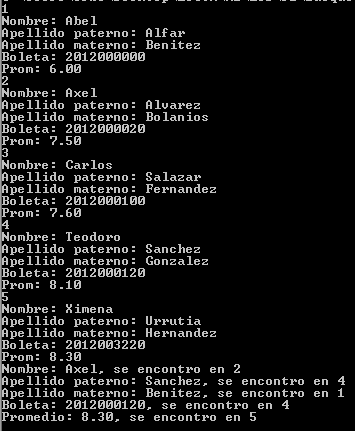
\includegraphics{Busqueda/img/TareaB_1.png}

\newpage
c) Programar la búsqueda por interpolación para una
lista de trabajadores que contiene los siguientes datos:
número de identificación (del 000 al 999), nombre, puesto
y sueldo. La llave en este caso es el número de identificación.
\lstinputlisting{Busqueda/TareaC.c}
Capturas de Pantalla de Busqueda/TareaC.c
\newline
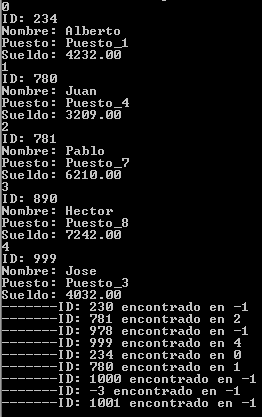
\includegraphics{Busqueda/img/TareaC_1.png}

\newpage
{\color[rgb]{1,0,0}
d) Hacer un programa de tablas hash abiertas. Las llaves
en este caso son número enteros largos. El programa debe
mostrar la manera en que queda la tabla después de insertar
o eliminar los elementos. Proponer la función hash a utilizar
y justificarla como comentario en el programa.
}

{\color[rgb]{1,0,0}
e) Hacer un programa de tablas hash cerradas. Las llaves
en este caso son número enteros largos. El programa debe
mostrar la manera en que queda la tabla después de insertar
o eliminar los elementos. Proponer las funciones hash a
utilizar y justificarla como comentario en el programa.
}

{\color[rgb]{1,0,0}
f) Se dispone de una aplicación de radares de tráfico que
permite llevar la contabilidad del número de veces que
ha pasado un determinado coche por dicho radar superando
el límite de velocidad. Para ello se consulta una lista
implementada mediante una Tabla Hash. Sabiendo que el
formato de una matrícula consta de una serie de 3 números
seguidos de 3 letras, hacer un programa que genere dicha
lista con el fin de contabilizar el número de veces que
ha pasado un coche; si es necesario, se debe actualizar la
lista de la aplicación. Si la matrícula no está en la lista
entonces el coche ha sido visto por primera vez. Si la
matrícula ya estaba en la lista entonces hay que guardar en
lista que se ha visto ese coche una vez más.
}
\newpage

{\center\Large\bfseries
\hspace*{45mm}
Tarea (recursión)
\newline
\newline
}
a) Resolver el problema de Las Torres de Hanoi
para cinco discos, mostrar la solución en forma
gráfica.
\lstinputlisting{Recursion/TareaA.c}
Capturas de Pantalla Recursion/TareaA.c
\newline
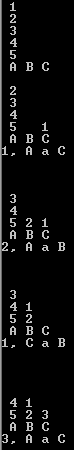
\includegraphics{Recursion/img/TareaA_1.png}
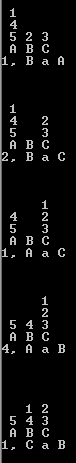
\includegraphics{Recursion/img/TareaA_2.png}
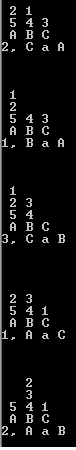
\includegraphics{Recursion/img/TareaA_3.png}
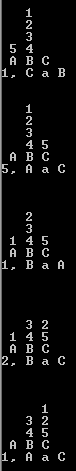
\includegraphics{Recursion/img/TareaA_4.png}
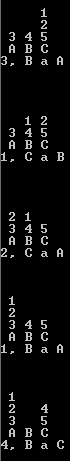
\includegraphics{Recursion/img/TareaA_5.png}
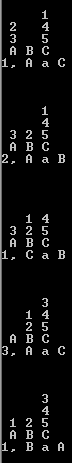
\includegraphics{Recursion/img/TareaA_6.png}
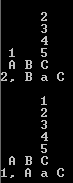
\includegraphics{Recursion/img/TareaA_7.png}
\newpage
b) Hacer un programa que, dados dos números, a (número entero)
y b (número natural mayor o igual que cero), determine
recursivamente $a^b$ (a elevado a la b).
\lstinputlisting{Recursion/TareaB.c}
Capturas de Pantalla Recursion/TareaB.c
\newline
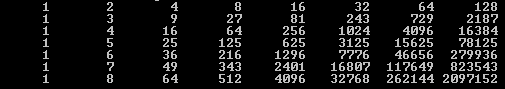
\includegraphics{Recursion/img/TareaB_1.png}
\newpage
{\color[rgb]{1,0,0}
c) Hacer un programa que, dados dos arreglos de números
enteros $A$ y $B$ de longitud $n$ y $m$ respectivamente, siendo
$n >= m$, determine resursivamente si $B$ está contenido en
$A$. Por ejemplo, si $A = \{2,3,4,5,8,9,-2\}$.
Si $B = \{9,-2\}$ está contenido, si $B = \{4,8\}$ no está
contenido, si $B = \{5,4\}$ no está contenido.
}

d) Suponga que $com(n,k)$ representa la cantidad de
diferentes comités de k personas que pueden formarse,
dadas n personas entre las cuales elegir. Por ejemplo,
$com(4,3) = 4$, porque dadas cuatro personas $A$,$B$,
$C$ y $D$ hay cuatro comités de tres personas posibles:
$ABC$, $ABD$, $ACD$ y $BCD$. Se puede comprobar la identidad:
\newline\hspace*{5mm}
$com(n,k) = com(n-1,k) + com(n-1,k-1)$
\newline
Escribir y probar un programa recursivo para calcular
$com(n,k)$ para $n,k >= 1$.
\lstinputlisting{Recursion/TareaD.c}
Capturas de Pantalla de Recursion/TareaD.c
\newline
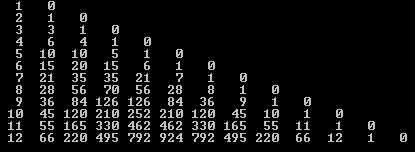
\includegraphics{Recursion/img/TareaD_1.png}
\newpage
e) Escribir un programa con una función recursiva que
acepte una expresión prefija que conste de operadores
binarios y operandos enteros de un solo dígito y
retorne el valor de la expresión.
\lstinputlisting{Recursion/TareaE.c}
Capturas de Pantalla de Recursion/TareaE.c
\newline
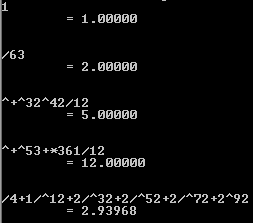
\includegraphics{Recursion/img/TareaE_1.png}

\newpage

{\center\Large\bfseries
\hspace*{45mm}
Tarea (árboles)
\newline
\newline
}
a) Hacer un programa para crear y manipular (hacer todas
las operaciones básicas) un árbol binario, haciendo una
implementación dinámica.
\lstinputlisting{Arboles/TareaA.c}
\newpage
{\color[rgb]{1,0,0}
b) Hacer un programa para crear y manipular (hacer todas
las operaciones básicas con) un árbol binario casi completo
utilizando un arreglo. Si el árbol no es casi completo, debe
hacerse y considerar nodos vacíos.
}

c) Hacer funciones para desplegar los árboles creados
en los incisos anteriores.
\lstinputlisting{Arboles/TareaC.c}
Capturas de Pantalla de Arboles/TareaC.c
\newline
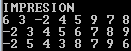
\includegraphics{Arboles/img/TareaC_1.png}

\newpage
d) Escribir funciones que permitan determinar:
\newline\hspace*{15mm}
a. La cantidad de nodos de un árbol binario.
\newline\hspace*{15mm}
b. La suma del contenido de todos los nodos en un
árbol binario.
\newline\hspace*{15mm}
c. La profundidad de un árbol binario.
\newline\hspace*{15mm}
d. El número de ocurrencias de un elemento en un
árbol binario.
\lstinputlisting{Arboles/TareaD.c}
Capturas de Pantalla de Arboles/TareaD.c
\newline
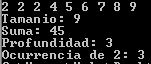
\includegraphics{Arboles/img/TareaD_1.png}

\newpage
e) Escribir un programa que acepte un apuntador a un
árbol binario y retorne un apuntador a un nuevo árbol
binario que sea la imagen reflejo del primero, es decir,
que todos los subárboles izquierdos sean ahora subárboles
derechos y viceversa.
\lstinputlisting{Arboles/TareaE.c}
Capturas de Pantalla de Arboles/TareaE.c
\newline
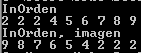
\includegraphics{Arboles/img/TareaE_1.png}
\newpage
f) Escribir un programa que realice el ordenamiento
de una serie de números, creando un árbol binario de
búsqueda y después el recorrido correspondiente.
\lstinputlisting{Arboles/TareaF.c}
Capturas de Pantalla de Arboles/TareaF.c
\newline
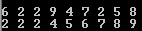
\includegraphics{Arboles/img/TareaF_1.png}
\newpage
{\color[rgb]{1,0,0}
g) Escribir un programa que construya un árbol de
expresión a partir de una cadena posfija.
}

{\color[rgb]{1,0,0}
h) Hacer un programa que convierta una expresión infija
a posfija mediante árboles.
}


\end{document}